\newcommand\N{\ensuremath{\mathbb{N}}} 
\newcommand\R{\ensuremath{\mathbb{R}}} 
\newcommand\A{\ensuremath{\mathbb{A}}} %affine space
\newcommand\Z{\ensuremath{\mathbb{Z}}} 
\renewcommand\O{\ensuremath{\emptyset}} 
\newcommand\Q{\ensuremath{\mathbb{Q}}} 
\newcommand\C{\ensuremath{\mathbb{C}}}
\newcommand\F{\ensuremath{\mathbb{F}}} %field
\newcommand\E{\ensuremath{\mathbb{E}}} %field extension
\renewcommand\P{\ensuremath{\mathbb{P}}} %projective space
\renewcommand\H{\ensuremath{\mathbb{H}}} %hyperbolic space
\newcommand\im{\ensuremath{\operatorname{im}}} %image
\newcommand\rank{\ensuremath{\operatorname{rank}}} %rank
\newcommand\id{\ensuremath{\operatorname{id}}} %identity map
\newcommand\grad{\ensuremath{\operatorname{grad}}} %gradient
\newcommand\curl{\ensuremath{\operatorname{curl}}} %gurl
\renewcommand\div{\ensuremath{\operatorname{div}}} %divergence
\newcommand\Gr{\ensuremath{\operatorname{Gr}}} %grassmannian
\newcommand\Hom{\ensuremath{\operatorname{Hom}}} %linear mappings

\documentclass[xcolor=dvipsnames]{beamer} 
\usetheme{Copenhagen} 
\beamertemplatenavigationsymbolsempty
\definecolor{burntorange}{RGB}{191,87,0}
\definecolor{utgrey}{RGB}{51,63,72} 

\setbeamercolor{palette primary}{bg=burntorange,fg=white}
\setbeamercolor{palette secondary}{bg=burntorange,fg=white}
\setbeamercolor{palette tertiary}{bg=burntorange,fg=white}
\setbeamercolor{palette quaternary}{bg=burntorange,fg=white}
\setbeamercolor{structure}{fg=burntorange} % itemize, enumerate, etc
\setbeamercolor{section in toc}{fg=burntorange} % TOC sections
\setbeamercolor{subsection in head/foot}{bg=burntorange,fg=white}
\setbeamercolor{block title example}{fg=white,bg=burntorange}
%\setbeamercolor{block body example}{fg=white,bg=burntorange}

\usepackage[utf8]{inputenc} 
\usepackage{float}
\usepackage{tikz} 
\usepackage{tikz-cd} 
\usepackage{amsmath, amssymb, amsthm}
\newtheorem{prop}{Proposition}[section]

\renewcommand\qedsymbol{$\boxtimes$}
\title{Bordism and TQFTs} 
\subtitle{A brief introduction to topological quantum field theories} 
\author{Simon Xiang} 
\institute{University of Texas at Austin} 
\begin{document} 
    \begin{frame}
        \titlepage
    \end{frame}

    \begin{frame}
\frametitle{Bordism} 
\begin{definition}[]
    Let $Y_0,Y_1$ be closed $n$-manifolds. A \textbf{bordism} $X$ from $Y_0$ to $Y_1$ is a compact $(n+1)$-manifold $X$ with boundary, a decomposition $\partial X= M_0 \amalg M_1$, and diffeomorphisms $\theta _i  \colon Y_i  \xrightarrow{\cong}  M_i $. 
\end{definition}
\begin{figure}[H]
\centering
 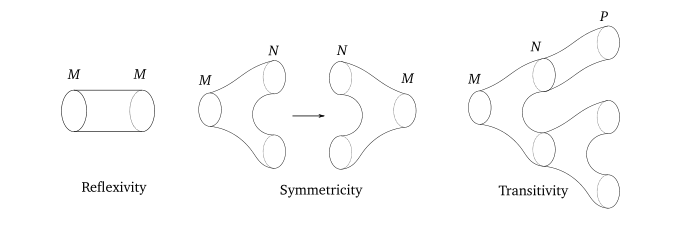
\includegraphics[width=0.6\linewidth]{figures/equivbord.png}
\end{figure}
\begin{definition}[]
    Let $\Omega_n $ denote the set of equivalence classes of $n$-manifolds under the equivalence relation of bordism. An element of $\Omega_n $ is called a \textbf{bordism class}.
\end{definition}
    \end{frame}

    \begin{frame}
        \frametitle{Bordism groups} 
        Disjoint union gives $\Omega_n $ a \emph{commutative monoid}  structure, and for  $Y \in \Omega_n $, the manifold $[0,1] \times Y$ is a bordism between $Y\amalg Y$ and the unit $\O^n $. So $\Omega_n $ is an \emph{abelian group}. 
        \begin{example}
           Some calculations:
           \begin{itemize}
               \item $\Omega_0 \cong \Z /2 \Z$ with generator $\mathrm{pt}$. Even points are bordant by intervals, and the single point cannot bound by classification.
               \item $\Omega_1 \cong 0$. Closed 1-manifolds are copies of circles which bound.
               \item $\Omega_2 \cong \Z/2\Z$ with generator $\R \mathrm P^2$. 
\begin{figure}[H]
\centering
\begin{minipage}[b]{0.5\linewidth} 
 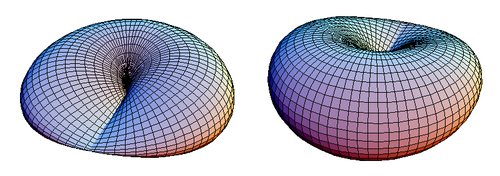
\includegraphics[width=0.8\linewidth]{figures/rp2.PNG}
\end{minipage}
\begin{minipage}[b]{0.4\linewidth} 
 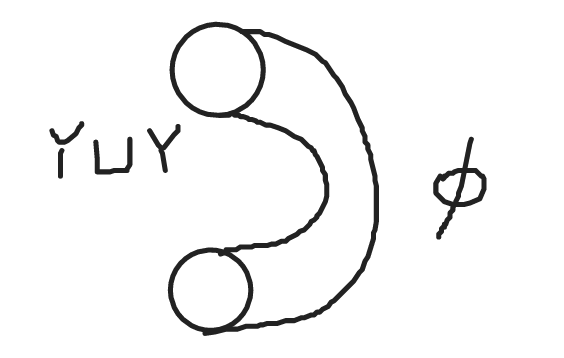
\includegraphics[width=0.7\linewidth]{figures/group.png}
\end{minipage}
\end{figure}
                   %Oriented surfaces are either 2-spheres or genus $g$ surfaces, which bound 3-balls and handlebodies. 
                   %Unoriented surfaces are connect sums of $\R \mathrm P^2$; and $M_0 \amalg M_1$ is bordant to $M_0 \# M_1$. $\R \mathrm P^2$ doesn't bound, and $\R \mathrm P^2\# \R \mathrm P^2$ is diffeomorphic to $K$ (which bounds). {\color{red}todo:get rid of text, add image instead} 
           \end{itemize}
        \end{example}
    \end{frame}

        \begingroup
        \small
    \begin{frame}[fragile]
        \frametitle{Symmetric monoidal categories} 
        \begin{definition}[Symmetric monoidal categories]
            Let $C$ be a category. A \textbf{symmetric monoidal structure} on $C$ consists of an object $1_C \in C$, a functor $\otimes \colon C\otimes C \to C$, and natural isomorphisms\[ 
    \begin{tikzcd}
        C\times C\times C\arrow[rr, "-\otimes(-\otimes -)", bend left] \arrow[rr, "(-\otimes -)\otimes -"', bend right] & \,\,~ \Big\Uparrow\alpha  & C
\end{tikzcd},
    \] \[
        \begin{tikzcd}
        C\times C\arrow[rr, "(-\otimes -)\circ \tau", bend left] \arrow[rr, "-\otimes -"', bend right] & \,\,~ \Big\Uparrow\sigma  & C
\end{tikzcd}, \quad \text{and} \quad
        \begin{tikzcd}
        C\arrow[rr, "\id_C", bend left] \arrow[rr, "1_C \otimes -"', bend right] & \,\,~ \Big\Uparrow\iota  & C
\end{tikzcd}.
    \]
           Some other compatibility axioms are required, like $\sigma^2=\id$, they essentially say that $\alpha ,\iota,$ and $\sigma$ behave well with each other. 
        \end{definition}
    \end{frame}

    \begin{frame}[fragile]
        \frametitle{Symmetric monoidal categories} 
        \begin{example}
            Consider $(\mathsf{Vect} _k,\otimes, k)$, then this is a symmetric monoidal category. Here $1_{\mathsf{Vect} _k}\in \mathsf{Vect} _k$ is $k$, the functor $\otimes \colon \mathsf{Vect} _k \otimes \mathsf{Vect} _k\to \mathsf{Vect} _k$ is the standard tensor product, and the natural isomorphisms exist.
        \end{example}
        \begin{definition}[Symmetric monoidal functors]
            Let $C,D$ be symmetric monoidal categories. A \textbf{symmetric monoidal functor} $F \colon C \to D$ is a functor with additional data, namely an isomorphism $1_D \to F(1_C)$ and a natural isomorphism \[
                   \begin{tikzcd}
            C\times C\arrow[rr, "F(-\otimes -)", bend left] \arrow[rr, "F(-)\otimes F(-)"', bend right] & \,\,~ \Big\Uparrow\psi  & C
\end{tikzcd}.
            \] and many compatibility conditions.
        \end{definition}
    \end{frame}
    \endgroup

\begin{frame}
    \frametitle{Bordism categories} 
    \begin{definition}[]
    Fix $n \in \Z^{\geq 0}$. The \textbf{bordism category} $\mathsf{Bord} _{\langle n-1,n \rangle }$ is the symmetric monoidal category defined as follows.
    \begin{enumerate}
\item Objects are closed $(n-1)$-manifolds.
\item The hom-set $\mathsf{Bord} _{\langle n-1,n \rangle }(Y_0,Y_1)$ is the set of diffeomorphism classes of bordisms $X \colon Y_0 \to Y_1$.
\item Composition of  morphisms is by gluing.
\item For each $Y$ the bordism $[0,1] \times Y$ is $\id_Y \colon Y \to Y$.
\item The monoidal product is disjoint union.
\item The empty manifold $\O ^{n-1}$ is the tensor unit (for the symmetric monoidal structure).
    \end{enumerate}
\end{definition}
\end{frame}

\begin{frame}
    \frametitle{Examples of bordism categories} 
    \begin{example}
        \begin{itemize}
            \item $\mathsf{Bord} _{\langle -1,0 \rangle }$ is a category with a single object $\O ^{n-1}$, hence a monoid, namely the set of morphisms $\mathsf{Bord} _{\langle -1,0 \rangle }(\O^{-1},\O^{-1})$. These are finite unions of points with diffeomorphism class $\Z ^{\geq 0}$, and composition/disjoint union both induce addition. 
            \item $\mathsf{Bord} _{\langle 0,1 \rangle }$ has objects points, with four distinct connected bordisms up to diffeomorphism.
                \begin{figure}[H]
                \centering
                 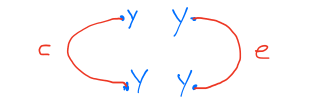
\includegraphics[width=0.6\linewidth]{../figures/evcoev.png}
                \end{figure}
        \end{itemize}
    \end{example}
\end{frame}

\begingroup
\small
\begin{frame}
    \frametitle{Duality} 
    \begin{definition}[Duality data]
  For a symmetric monoidal category $C$ and $y \in C$, we say $y$ is \textbf{dualizable} if there exists \emph{duality data} $(y ^{\vee},c,e)$, where $y ^{\vee} \in C$, $c \colon 1_C \to y \otimes y ^{\vee}, e \colon  y^{\vee}\otimes y \to 1_C$, such that
        \begin{gather}
            \left( y \xrightarrow{c\otimes\id_y} y\otimes y^{\vee}\otimes y\xrightarrow{\id_y \otimes e}y \right)=\id_y ,\\
        \left( y ^{\vee}\xrightarrow{\id_{y^{\vee}} \otimes c} y ^{\vee}\otimes y \otimes y ^{\vee}\xrightarrow{e \otimes \id_{y ^{\vee}} } y ^{\vee}\right)         =\id _{y ^{\vee}}.
    \end{gather}
    \end{definition}
    \begin{example}
        Recall ``evaluation'' and ``coevaluation'' from $\mathsf{Bord}_{\langle 0,1 \rangle } $. 
        \begin{figure}[H]
        \centering
         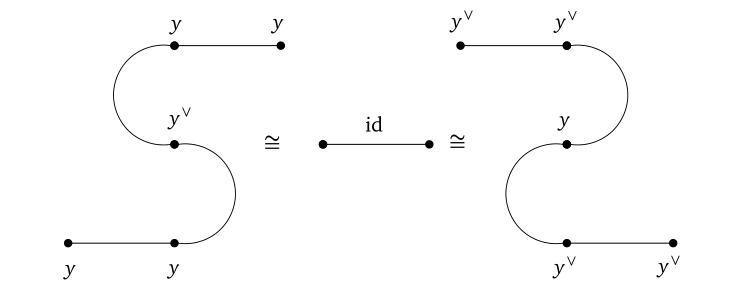
\includegraphics[width=0.5\linewidth]{figures/szdiagram.png}
        \end{figure}
    \end{example}
\end{frame}


\begin{frame}
\frametitle{Duality in vector spaces} 
    %\begin{definition}[Dual morphism]
        %For $y_0,y_1$ dualizable and $f \colon y_0 \to y_1$, we have the \textbf{dual morphism} $f ^{\vee} \colon y_1 ^{\vee} \to y_0 ^{\vee}$ given by the composition \[
            %y_1 ^{\vee}\xrightarrow{\id _{y_1^{\vee}}\otimes c_0} y_1 ^{\vee}\otimes y_0 \otimes y_0 ^{\vee}\xrightarrow{\id_{y_1^{\vee}}\otimes f \otimes \id_{y_0 ^{\vee}} } y_1 ^{\vee }\otimes y_1 \otimes y_0 ^{\vee}\xrightarrow{e_1 \otimes \id _{y_0 ^{\vee}}} y_0^{\vee}
        %\] 
    %\end{definition}
    \begin{example}
%        Let $V,W \in  \mathsf{Vect} _k$ and  $T \colon V \to W;$ we have the pullback $T^* \colon W^* \to V^*$ given by $(T^*f)(v) := f(T(v))$. We also have 
        Let $V \in \mathsf{FdVect} _k$. Then we have duality data consisting of the algebraic dual $V^*$, along with the following maps:
        \begin{itemize}
    \item $e \colon V^* \otimes V \to k, (f,v) \mapsto  f(v)$ (evaluation)
    \item $c \colon k \to V \otimes V^*, \lambda \mapsto \sum_i  \lambda v_i  \otimes v_i ^* $ (coevaluation)
        \end{itemize}
 %Sending a covector through the dual morphism composition, we get \[
        Send a vector  $v_j  \in V$ and a covector $f\in  V^*$ through the duality data:
 \begin{gather*}
     v_j  \to \left( \sum _i  v_i  \otimes v_i ^* \right) \otimes v_j \to \sum _i  v_i \otimes \delta ^i _j =v_j ,\\
     f \to f\otimes \left( \sum _i  v_i  \otimes v_i ^* \right) \to \sum _i  f(v_i )\otimes v_i ^*=f.
 \end{gather*}
 We need $V$ to be \emph{finite dimensional}  because otherwise we cannot write down coevaluation, which requires a basis.
     %f \to  f \otimes \sum _i  v_i \otimes v_i  ^* \to f \otimes \sum T(v_i )\otimes v_i ^* \to \sum _i  f(T(v_i ))\otimes v_i ^*
 %As $v_i ^*=\delta^i _j  $, evaluating on $v_j \in  V$, we get $\sum _i  f(T(v_i )) \otimes \delta ^i_j =f(T(v_j ))$, precisely the pullback. {\color{red}todo:ask about eval, basis (FD). vector space dualizable iff FD, write down eval, coev (can't write down coev if infinite dim)} 

    \end{example}
\end{frame}
\endgroup

\begin{frame}
    \frametitle{TQFTs} 
    \begin{definition}[Topological quantum field theories]
        Let $C$ be a symmetric monoidal category. Then an $\mathbf n$\textbf{-dimensional topological quantum field theory} with values in $C$ is a symmetric monoidal functor \[
        F \colon \mathsf{Bord} _{\langle n-1,n \rangle } \to C
        \] Usually we consider $\mathsf{Vect} _k$ for $k = \C$.
    Note that $n$-dimensional TQFTs form a symmetric monoidal category $\mathsf{TQFT} _n $ under the natural tensor product.
    \end{definition}  
    %qft: notion of space and time. $(n-1)$-manifold as cutting spacetime at a particular time. vector space is the vector space of states (possible configurations), bordism represents evolution. partition function value of theory on manifold
    %\begin{example}
        %Let $M$ be a closed $k$-manifold, then there is a ``TQFT'' $- \times M \colon \mathsf{Bord} _{\langle n-1,n \rangle } \to \mathsf{Bord}_{\langle n-1+k,n+k \rangle }$; precomposing with any $(n+k)$-dimensional TQFT reduces its dimension by $k $ to $n$.
    %\end{example}
\end{frame}

\begin{frame}
   \frametitle{More on TQFTs}  

   \begin{example}
      A closed $n$-manifold $M$ can be seen as a bordism $\O ^{n-1}\to \O^{n-1}$, under a TQFT $F$ this gets send to an endomorphism of $k$, or a number. 
   \end{example}
   \begin{prop}[Finiteness]
       Let $F \colon \mathsf{Bord} _{\langle n-1,n \rangle } \to \mathsf{Vect} _{\C}$ be a TQFT. Then for all $Y \in \mathsf{Bord} _{\langle n-1,n \rangle }$, $F(Y)$ is finite dimensional.
   \end{prop}
   \begin{proof}
       Note that a point (manifold) in $\mathsf{Bord} _{\langle n-1,n \rangle }$ is dualizable. Symmetric monoidal functors preserve duality data, so the vector space $F(Y)$ is dualizable, which is true iff $F(Y)$ is finite dimensional.\qedhere
   \end{proof}
\end{frame}

\begin{frame}
    \frametitle{Classification of 1-dimensional TQFTs} 
    \begin{definition}[Categorical stuff]
        Let $C$ be a symmetric monoidal category. Define $C ^{\mathrm{fd}}$ as the full subcategory of dualizable objects, and the \emph{groupoid of units} $C ^{\sim}$ containing only invertible morphisms.
    \end{definition}
    \begin{theorem}[Cobordism hypothesis, 1-categorical version] 
       Let $C$ be a symmetric monoidal category. Then the map \[
           \Phi \colon \mathsf{TQFT}^{\mathrm{or}}_{\langle 0,1 \rangle }(C) \to (C ^{\mathrm{fd}}) ^{\sim}, \quad F \mapsto F ( \mathrm{pt}_+)
       \]  is an equivalence of groupoids.

       %{\color{red}todo:section of oriented double cover, non-vanishing 1-form (sends to 1) (linear functional on the tangent space, sections of cotangent bundle). what is positively oriented point? 2-3:30} 
    \end{theorem}
    
    %{\color{red}idea is that bord 0,1 is generated by point and duality data (circle?). tqft is equiv to fd vect with non-degen bilinear map. get to a thm (classification of 1d tqfts?)} 
\end{frame}

\end{document}
